\documentclass[a4paper,14pt,twoside]{extarticle} \usepackage[utf8]{inputenc}
\usepackage[T1]{fontenc}
\usepackage[margin=2.5cm]{geometry}

% Fonte Caladea se existir, senão lmodern
\IfFileExists{caladea.sty}{
  \usepackage{caladea}
}{
  \usepackage{lmodern} }
\usepackage{ragged2e}
\usepackage{graphicx}
\usepackage[portuguese]{babel}
\usepackage{wrapfig}
\usepackage{hyperref}
\usepackage{fancyhdr}
\usepackage{xcolor}
\usepackage{rotating}
\usepackage{titlesec}
\usepackage{epigraph}
\usepackage{dirtytalk}
\usepackage{indentfirst} % Indenta o primeiro parágrafo após seções

% Ajuste do recuo de parágrafo
\setlength{\parindent}{1.5em}

% Centralizar títulos
\titleformat{\section}
  {\normalfont\centering\bfseries\Large}{\thesection}{1em}{}

\titleformat{\subsection}
  {\normalfont\centering\bfseries\large}{\thesubsection}{1em}{}

\titleformat{\subsubsection}
  {\normalfont\centering\bfseries}{\thesubsubsection}{1em}{}

% -------------- Símbolos de Versículo e Resposta --------------
% Definição do símbolo (a “barrinha” inclinada)
\makeatletter
\newcommand{\vers@resp@sym}{%
  \raisebox{0.2ex}{\rotatebox[origin=c]{-20}{$\m@th\rceil$}}%
}
% macro interna que sobrepõe a barrinha e a letra V ou R
\newcommand{\vers@resp}[2]{%
  {\ooalign{%
     \hidewidth\kern#1\vers@resp@sym\hidewidth\cr
     #2\cr
  }}%
}
% comandos públicos \versicle e \response
\DeclareRobustCommand{\versicle}{\vers@resp{-0.1em}{\textbf{V}}}
  \DeclareRobustCommand{\response}{\vers@resp{0pt}{\textbf{R}}}
\makeatother
% ^------------- Símbolos de Versículo e Resposta -------------^

% Rodapé com imagem e página
% Ajuste para cabeçalho do fancyhdr
\setlength{\headheight}{18pt} % Ajuste recomendado pelo warning do fancyhdr
\pagestyle{fancy}
% ---- Cabeçalho ------------
\fancyhf[C]{}
% ----- Rodapé --------------
\fancyfoot[LO,LE]{%
  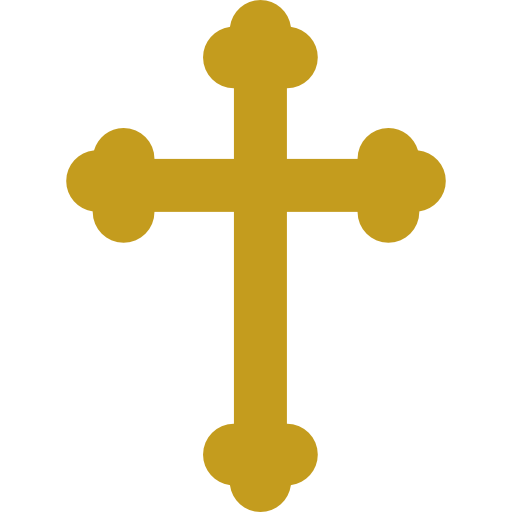
\includegraphics[scale=0.2]{assets/cross.png}\quad
  \textit{Novena a \textbf{Santo Alberto Magno}}
}
\fancyfoot[RO,RE]{\thepage}

\begin{document}


\begin{center}
  {\huge Novena a Santo Alberto Magno}
\end{center}


\say{A vida de Santo Alberto Magno prova, que todo o saber vem de Deus. Se temos talentos, deles não nos devemos orgulhar, porque de Deus é que os recebemos. Se o mundo nos admira, bate aplausos aos nossos trabalhos, a Deus é que pertence esta glória, a Deus, que é sabedoria eterna e o doador de todos os bens. Nada somos e nada temos. Se a Deus toda a glória e honra devemos dar, não menos certo é que dos talentos que nos foram confiados, e do uso que deles fizemos um dia havemos de prestar contas ao Juiz eterno.}


{\centering \rule{1.0\textwidth}{0.4pt}}

\tableofcontents
\thispagestyle{empty}


\newpage
\section{História}

Alberto nasceu na Alemanha, por volta de 1200, no seio de uma família de condes, Bollstadt. Ao crescer, foi enviado para estudar em Pádua, uma cidade excelente de artes liberais, mas também em Bolonha e Veneza.
Como jovem estudante, era realmente brilhante, mas quando foi chamado para aprofundar o estudo de Teologia, em Colônia, encontrou muitas dificuldades, a ponto vacilar na fé. Sua salvação foi a grande devoção que nutria pela Virgem, que nunca o abandonou.

\subsection{Chamada para a Ordem dos Pregadores}

Na Itália, Alberto conheceu os Padres Dominicanos, a Ordem dos Pregadores, e percebeu que era aquela a sua estrada: recebeu o hábito religioso das mãos do Beato Jordano da Saxônia, sucessor imediato de São Domingos. Assim, foi enviado, primeiro, a Colônia e, depois, a Paris, onde, por alguns anos, ocupou a cátedra de Teologia e também conheceu seu aluno mais talentoso: Tomás de Aquino, que o levou consigo quando a Ordem o enviou, novamente, a Colônia, para dar início ao estudo teológico.
Amor pelo ensino e o encontro com Tomás

O ensino foi a maior paixão de Alberto, depois daquela pelo Senhor. Em Colônia, junto com Tomás, conseguiu fazer grandes coisas, tanto que recebeu o apelido de "Magno", isto é, Grande. Ambos empreenderam o ambicioso projeto de comentar a obra de Dionísio, o Areopagita, e os escritos de Aristóteles sobre filosofia natural.
Desta forma, Alberto conseguiu descobrir o ponto de encontro entre os dois grandes estudiosos da antiguidade sobre a doutrina da alma: colocada por Deus na obscuridade do ser humano, ela se expressa no conhecimento e, precisamente nesta atividade complexa e maravilhosa, revela a sua natureza e a sua origem divina. Com esta síntese, entre a sabedoria dos Santos, o conhecimento humano e a ciência da natureza, Alberto deu um profundo impulso à orientação mística da Ordem, à qual pertencia, confiando a pesquisa filosófico-teológica ao fiel Tomás.

\subsection{Em Roma, com o Papa}

No Capítulo Geral dos Dominicanos, que se realizou em Valenciennes, em 1250, Alberto elaborou, com Tomás, normas para a direção dos estudos e a determinação do sistema de méritos no âmbito da Ordem. Por isso, quatro anos depois, deixou o ensino e foi "promovido" como Provincial na Alemanha.
Com este cargo, em 1256, foi a Roma para defender os direitos da Santa Sé e dos religiosos Mendicantes no Consistório de Anagni. O Pontífice ficou tão impressionado com ele, que o mandou ficar na cidade e a retomar o ensino, que tanto amava, atribuindo-lhe uma cátedra na Universidade Pontifícia.

\subsection{Na cátedra, como Bispo, e seus últimos anos}

Por sua surpresa, em 1260, o Papa nomeou Alberto novo Bispo de Regensburg. Ao voltar à sua pátria, o Santo empenhou-se, como assiduidade, para fortalecer a paz entre os povos.
Em 1274, o Papa Gregório X convidou-o, novamente, a participar do segundo Concílio de Lyon, mas, no caminho de volta, recebeu uma notícia, que jamais queria receber: o falecimento de Tomás, um duro golpe para Alberto, que o amava como um filho, sobre o qual teve apenas a força de comentar: "A luz da Igreja se apagou".
Por isso, começou a pedir, com insistência, a Urbano IV, para isentá-lo do cargo pastoral e se retirar para Colônia. E o Papa lhe permitiu.
Continuando a escrever e a rezar, Alberto faleceu em 15 de novembro de 1280. Pio XI o canonizou em 1931 e o proclamou Doutor da Igreja. Dez anos depois, Pio XII o declarou Padroeiro dos cultores de Ciências naturais.

% --- Orações Diárias ---
\newpage

\section{Novena a Santo Alberto Magno}

Altíssimo e onipotente Deus, conceda-nos um espírito aberto e compreensivo como aquele que destes a Santo Alberto. Dá-nos a graça de penetrar em teus mistérios com nossa inteligência, a fim de que tudo isso nos conduza a iniciarmos uma vida de oração constante e agradável em tua presença. 

Ó São Alberto Magno, sábio doutor da Igreja e patrono dos que buscam o conhecimento na luz da fé, a ti recorremos em nossa busca por sabedoria e entendimento. Tu que dedicaste tua vida à exploração das maravilhas da criação de Deus, guiando-se sempre pela luz da razão e da fé, intercedei por nós junto ao Senhor.

Rogamos que, por tua intercessão, sejamos abençoados com a curiosidade intelectual e a clareza de pensamento que marcaram tua jornada terrena. Que possamos encontrar, enfim, a harmonia entre a ciência e a fé, reconhecendo o trabalho do Criador em cada partícula do universo.

Ensinai-nos a buscar a verdade em todas as coisas, com humildade e dedicação. Que o amor pelo aprendizado e a paixão pela investigação da natureza nos aproximem cada vez mais do Divino.

Ó mestre de santos e guia dos tantos estudiosos, por tua sabedoria, foste capaz de iluminar muitas mentes e corações. Ajuda-nos a utilizar nosso conhecimento para o bem da humanidade, promovendo a paz, a justiça e o respeito mútuo entre todos os povos.

Seguindo teus passos, possamos contribuir para a construção de um mundo mais justo e fraterno, onde o amor de Deus seja manifestado através de nossas ações e descobertas.

Intercedei também por nossas necessidades particulares: (\textbf{mencione as intenções aqui})

\versicle. Rogai por nós, Santo Alberto Magno,

\response. Para que sejamos dignos das promessas de Cristo.

\vfill

\begin{center}
\subsection*{Fontes:}
Adaptado de: 
 \underline{\href{https://www.vaticannews.va/pt/santo-do-dia/11/15/s--alberto-magno--bispo-e-doutor-da-igreja--dominicano.html}{Vatican News}} e  \underline{\href{https://cruzterrasanta.com.br/santo-alberto-magno/181/105/}{Cruz Terra Santa}}.
\end{center}


\end{document}
